\documentclass[../main]{subfiles}
\begin{document}

\chapter{模拟乘法混频}%
\label{cha:模拟乘法混频}

\section{实验目的}%
\label{sec:\arabic{chapter}实验目的}

\begin{enumerate}

	\item 了解集成混频器的工作原理;

	\item 了解混频器中的寄生干扰。

\end{enumerate}

\section{基本原理}%
\label{sec:\arabic{chapter}基本原理}

在高频电子电路中,常常需要将信号自某一频率变成另一个频率。这样不仅能满足各种无线
电设备的需要,而且有利于提高设备的性能。对信号进行变频,是将信号的各分量移至新的
频域,各分量的频率间隔和相对幅度保持不变。进行这种频率变换时,新频率等于信号原来
的频率与某一参考频率之和或差。该参考频率通常称为本机振荡频率。本机振荡频率可以是
由单独的信号源供给,也可以由频率变换电路内部产生。当本机振荡由单独的信号源供给时
,这样的频率变换电路称为混频器。

混频器常用的非线性器件有二极管、三极管、场效应管和乘法器。本振用于产生一个等幅的
高频信号$ V_\mathrm{L} $,并与输入信号$ V_\mathrm{S} $经混频器后所产生的差频信号
经带通滤波器滤出。

本实验采用集成模拟相乘器作混频电路实验。

因为模拟相乘器的输出频率包含有两个输入频率之差或和,故模拟相乘器加滤波器,滤波器
滤除不需要的分量,取和频或者差频二者之一,即构成混频器。

\begin{figure}[htbp]
	\centering
	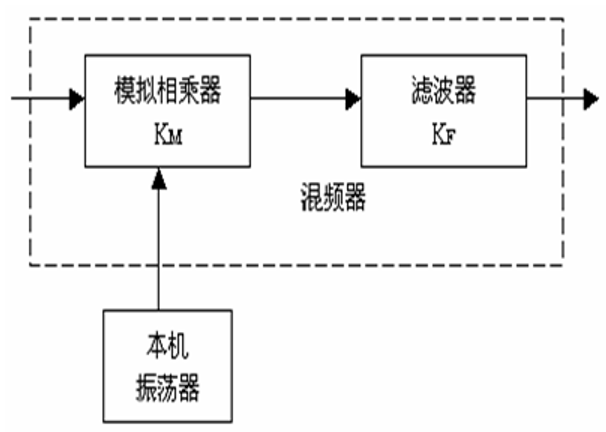
\includegraphics[width=0.8\linewidth]{block.png}
	\caption{相乘混频器方框图}
	\label{fig:相乘混频器方框图}
\end{figure}

\begin{figure}[htbp]
	\centering
	\begin{subfigure}[htbp]{.45\linewidth}
		\centering
		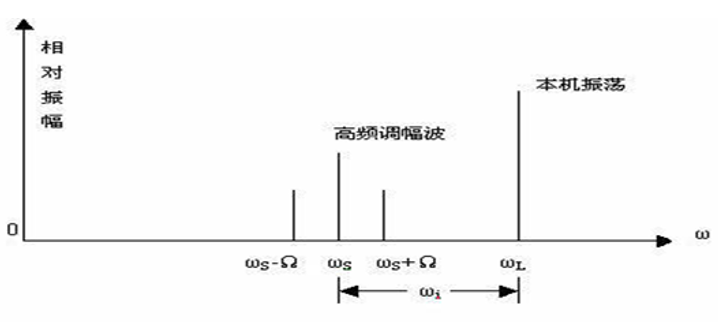
\includegraphics[width=\linewidth]{before.png}
		\caption{混频前的频谱图}
		\label{fig:混频前的频谱图}
	\end{subfigure}
	\quad
	\begin{subfigure}[htbp]{.45\linewidth}
		\centering
		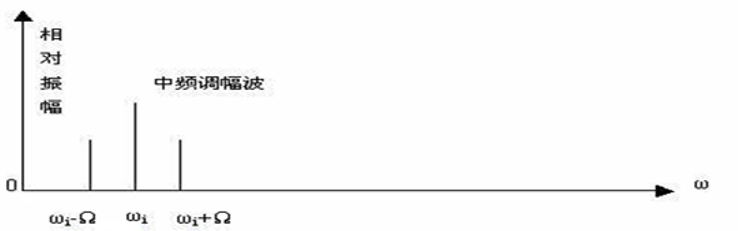
\includegraphics[width=\linewidth]{after.png}
		\caption{混频后的频谱图}
		\label{fig:混频后的频谱图}
	\end{subfigure}
	\caption{混频前后的频谱图}
	\label{fig:混频前后的频谱图}
\end{figure}

图\ref{fig:相乘混频器方框图}所示为相乘混频器的方框图。设滤波器滤除和频,则输出差
频信号。图\ref{fig:混频前后的频谱图}为信号经混频前后的频谱图。我们设信号是:载波
频率为$ f_\mathrm{S} $的普通调幅波。本机振荡频率为$ f_\mathrm{L} $。

\begin{figure}[htbp]
	\centering
	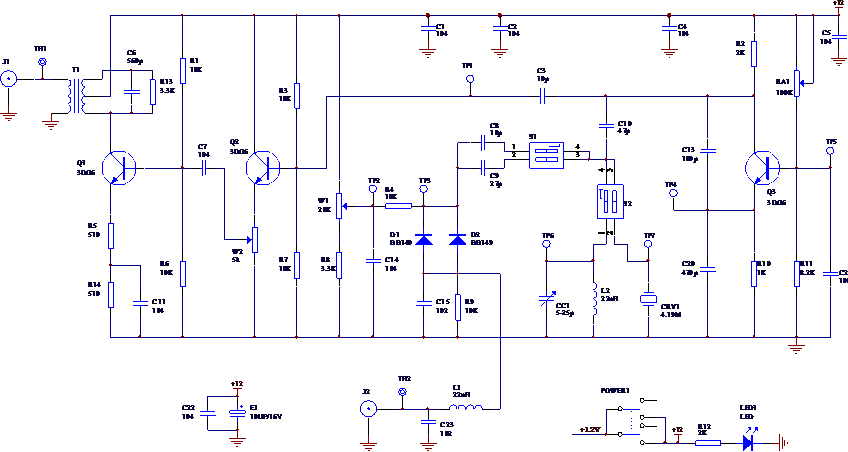
\includegraphics[width=0.8\linewidth]{circuit.png}
	\caption{模拟乘法器混频电路}
	\label{fig:模拟乘法器混频电路}
\end{figure}

图\ref{fig:模拟乘法器混频电路}为模拟乘法器混频电路,该电路由集成模拟乘法器MC1496
完成。MC1496可以采用单电源供电,也可采用双电源供电。本实验电路中采用\SI{+12}{\V}
,\SI{-8}{\V} 供电。$ R_{22} $(\SI{820}{\ohm})、$ R_{23} $(\SI{820}{\ohm})组
成平衡电路,$ F_2 $为\SI{4.5}{\MHz}选频回路。本实验中输入信号频率为
\SI{4.2}{\MHz},本振频率\SI{8.7}{\MHz},分别从$ J_3 $,$ J_4 $口输入。

\section{实验步骤}%
\label{sec:\arabic{chapter}实验步骤}

\begin{enumerate}

	\item 打开本实验单元的电源开关,观察对应的发光二极管是否点亮,熟悉电路各
		部分元件的作用。

	\item 用实验箱的信号源做本振信号,将频率\SI{8.7}{\MHz}(幅度$
		V_\mathrm{LP-P} = \SI{300}{\mV} $ 左右)的本振信号从$ J_3 $口处
		输入(本振输入处),在相乘混频器的输出端$ J_5 $口处观察输出中频
		信号波形,$ \mathrm{TH}_6 $处测试观察。

	\item 将(1号板提供)的晶体振荡频率\SI{4.19}{\MHz}(幅度$
		V_\mathrm{SP-P} = \SI{150}{\mV} $ 左右)的高频信号从相乘混频器的
		输入端$ J_4 $口输入,用示波器观察输出端$ J_5 $口处中频信号波形的
		变化,$ \mathrm{TH}_6 $ 处测试观察。

	\item 用示波器观察$ \mathrm{TH}_7 $和$ \mathrm{TH}_6 $处波形。

		\begin{figure}[htbp]
			\centering
			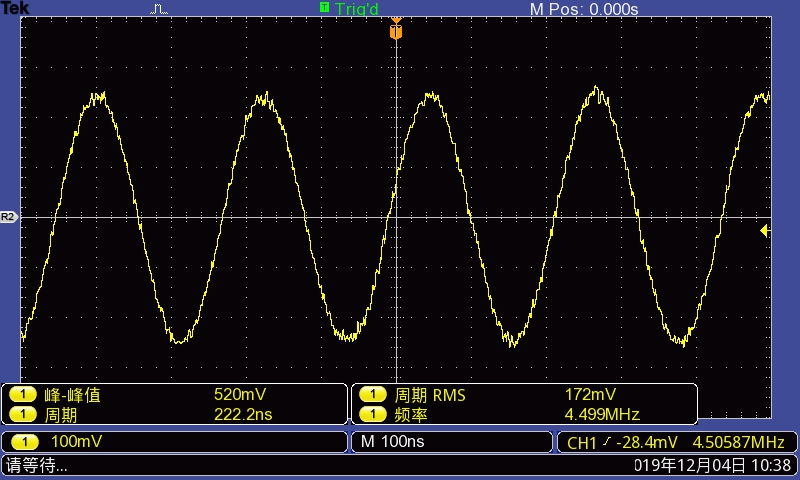
\includegraphics[width = 0.8\linewidth]{1.jpg}
			\caption{TH$ _7 $}
			\label{fig:TH7}
		\end{figure}

		\begin{figure}[htbp]
			\centering
			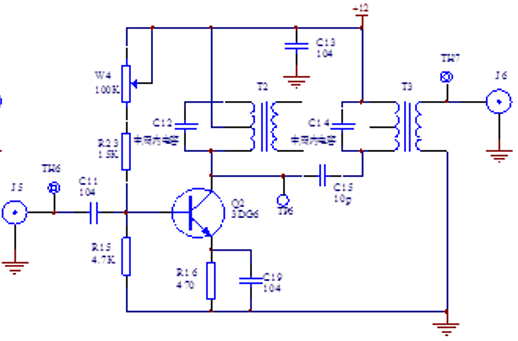
\includegraphics[width = 0.8\linewidth]{2.jpg}
			\caption{TH$ _6 $}
			\label{fig:TH6}
		\end{figure}

	\item 改变高频信号电压幅度,用示波器观测,记录输出中频电压$ V_\mathrm{i}
		$的幅值,并填入表\ref{tab:改变高频信号电压幅度}。

		\begin{table}[htbp]
			\centering
			\caption{改变高频信号电压幅度}
			\label{tab:改变高频信号电压幅度}
			\csvautobooktabular{tab/\arabic{chapter}/1.csv}
		\end{table}

	\item 改变本振信号电压幅度,用示波器观测,记录输出中频电压$ V_\mathrm{i}
		$的幅值,并填入表\ref{tab:改变本振信号电压幅度}。

		\begin{table}[htbp]
			\centering
			\caption{改变本振信号电压幅度}
			\label{tab:改变本振信号电压幅度}
			\csvautobooktabular{tab/\arabic{chapter}/2.csv}
		\end{table}

	\item 用频率计测量混频前后波形的频率。

	\item 混频的综合观测(需外接信号源)选作令高频信号发生器输出一个由
		\SI{1}{\kHz}音频信号调制的载波频率为\SI{4.2}{\MHz}的调幅波,作为
		本实验的载波输入,外接信号源输出\SI{8.7}{\MHz}的本振信号,用示波
		器对比观察$ J_5 $处和调制信号的波形。

\end{enumerate}

\section{实验报告要求}%
\label{sec:\arabic{chapter}实验报告要求}

\begin{Exercise}

	整理实验数据,填写表格\ref{tab:改变高频信号电压幅度}和
	\ref{tab:改变本振信号电压幅度}。

\end{Exercise}

\begin{Answer}

	实验数据见表\ref{tab:改变高频信号电压幅度}和
	\ref{tab:改变本振信号电压幅度}。

\end{Answer}

\section{实验仪器}%
\label{sec:\arabic{chapter}实验仪器}

\begin{table}[htbp]
	\centering
	\caption{实验仪器}
	\label{tab:\arabic{chapter}实验仪器}
	\csvautobooktabular{tab/\arabic{chapter}/BOM.csv}
\end{table}

\end{document}

